\documentclass[11pt]{article}

\usepackage{cvpr}
\usepackage{times}
\usepackage{epsfig}
\usepackage{graphicx}
\usepackage{caption}
\usepackage{subcaption}
\usepackage{amsmath}
\usepackage{amssymb}


% Change subsections from numerical to alphabetical
\renewcommand{\thesubsection}{\thesection.\alph{subsection}}


\cvprfinalcopy % *** Uncomment this line for the final submission

\begin{document}


\title{
	\large Image Processing - CSCE 5683\\
	Midterm Exam\\
	Fall 2018
}

\author{
	Reid Sutherland\\
	Masters - CS}

\maketitle



%%%%% Problem 1
\section{Question 1 - [8 pts]}
\textbf{Consider two 8-bit images whose intensity levels span the full range from 0 to 255.}\\

\subsection{Discuss the limiting effect of repeatedly subtracting image b from image a. Assume that the result is represented also in 8 bits. [Note: you can consider that when the gray level is negative it is assigned to zero]}
\begin{it}
For the remainder of this question, I will refer to image a as $A$ and image b as $B$.
\end{it}\\
\\
Since the images are 8-bits, we know they are both grayscale images from 0 to 255. Mathematically, the limit of $A(x,y) - B(x,y)$ is zero for all non-zero pixels. This is obvious, since if we subtract any non-zero number from any other number enough times, without going past zero, then we will eventually reach zero. As the subtraction operation described above is repeated, the resulting image will get darker and darker, eventually becoming a nearly all-black image. Based on the question's assumption, each pixel will approach 0 by the same amount with each pass, stopping at 0, which means that (almost) all pixels will eventually become black.\\
\\
The exception here is every pixel of $B$ where the value is 0. If we subtract 0 from a non-zero number, then that number will never change. Therefore, even if we subtract $B$ from $A$ an infinite number of times, $A$ will still have individual pixels that retain their original value, at every $(x, y)$ coordinate where $B(x, y) = 0$. All other pixels will eventually fade to black.\\
\\
As for the rate at which this occurs, each pixel $A(x,y)$ will fade at a static rate, where the rate is equal to the value of $B(x,y)$. In essence, $A(x,y)$ will fade more quickly (i.e., will approach black more rapidly with respect to the number of subtractions done) when $B(x,y)$ is larger. The inverse of this is true as well, $A$ pixels will fade more slowly when their corresponding $B$ pixels are smaller.


\subsection{Would reversing the order of the images, i.e. subtracting imagea from image b yield the same result? Explain.}
The same effect would be achieved, but the set of results would of course be different than Part (a), since rather than starting from $A$ and subtracting $B$, we would be starting with $B$ and subtracting $A$ each time. The behavior of the change in $B$ would be symbolically identical to the behavior of the change in $A$ in the last problem. The practical difference comes from the fact that $A$ and $B$ have different values, so obviously each operation $B(x,y) - A(x,y)$ would have a different result than the $A(x,y) - B(x,y)$ operations from the previous problem.



%%%%% Problem 2
\section{Question 2 - [12 pts]}

\subsection{Write down a 3 by 3 spatial filter mask that averages the four diagonal elements of a point (x, y) and the point itself. Find the corresponding filter H(u,v) in the frequency domain of this filter. Explain what this filter can do.}
Assuming, of course, that the center element of the filter mask represents each point (x, y):
\[
h(x,y) = \frac{1}{5}
\begin{bmatrix}
1 & 0 & 1\\
0 & 1 & 0\\
1 & 0 & 1\\
\end{bmatrix}
\]

To compute the frequency domain variant of this filter, $H(u,v)$, we simply calculate the product of each element of the spatial filter by a constant conversion factor. The conversion factor essentially represents the point by point conversion from the spatial domain to the overall frequency domain.
\[
\begin{split}
H(u,v) & = \sum_{x=-1}^{1} \sum_{y=-1}^{1} h(x,y) e^{-j2 \pi (xu + yv)} \\
& = \frac{1}{5} (1 + e^{-j2 \pi u} + e^{j2 \pi u} + e^{-j2 \pi v} + e^{j2 \pi v} ) \\
\end{split}
\]
Finally, we end up with the frequency filter:
\[
H(u,v) = \frac{1}{5} + \frac{1}{5}\cos(2 \pi u) + \frac{1}{5}\cos(2 \pi v)
\]
This filter is essentially a blurring kernel. By setting each pixel to the average of it and its neighbors, this will blur the entire image, but only slightly. This may be useful for increasing the distant quality of very low-resolution images.

\subsection{Write down a 3 by 3 Laplacian filter in the spatial domain. Find the corresponding filter H(u,v) in the frequency domain. Explain what this filter can do.}
\[
h(x, y) =
\begin{bmatrix}
1 & 0 & 1\\
0 & -4 & 0\\
1 & 0 & 1\\
\end{bmatrix}
\]
To compute the same laplacian filter in the frequency domain, we use the same process as on the previous question.
\[
\begin{split}
H(u,v) & = \sum_{x=-1}^{1} \sum_{y=-1}^{1} h(x,y) e^{-j2 \pi (xu + yv)} \\
& = -4 + e^{-j2 \pi u} + e^{j2 \pi u} + e^{-j2 \pi v} + e^{j2 \pi v} \\
\end{split}
\]
Finally, we end up with the laplacian frequency filter:
\[
H(u,v) = -4 + \cos(2 \pi u) + \cos(2 \pi v)
\]
This laplacian filter is essentially an edge detection kernel. Sharp (non-blurry), distinct edges in the foreground of the image should be highlighted, as if drawn with a white pencil, and everything else should be black or very dark. Gradual gradients of color shift (even relatively quick ones) would not be highlighted in this way.

\subsection{Show that the Fourier transform of the convolution of two functions is equal to the product of the Fourier transforms of the two functions. Give one example of the use of this result.}

%%%%% TODO
This problem asks the question that is solved by the Convolution Theorem. To showcase this theorem, I will demonstrate the proof here. First, let $F$ be the Fourier transformation of one function $f$, and let $G$ be the Fourier transformation of another function $g$.
\[
F(v) = Fourier(f) = \int_{\mathbb{R}^n} f(x) e^{-2 \pi ix \cdot v} dx
G(v) = Fourier(g) = \int_{\mathbb{R}^n} g(x) e^{-2 \pi ix \cdot v} dx
\]
Note that $x \cdot v$ refers to the inner product of $\mathbb{R}^n$. Now let $h$ be the convolution of $f$ and $g$.
\[
h(z) = \int_{\mathbb{R}^n} f(x) g(z - x) dx
\]
Therefore, we can assume the following equation:
\[
\begin{aligned}
\int \int | f(x) g(z - x) | dz dx  & = \int | f(x) | \int |g(z - x)| dz dx \\
& = \int | f(x) | ||g||_1 dx \\
& = \int ||f||_1 ||g||_1
\end{aligned}
\]
Now, thanks to Fubini's Theorem, we can define the Fourier Transform of $h$ as:
\[
\begin{aligned}
H(v) = Fourier(h) & = \int_{\mathbb{R}^n} h(z) e^{-2 \pi i z \cdot v} dz \\
& = \int_{\mathbb{R}^n} \int_{\mathbb{R}^n} f(x) g(z - x) dx e^{-2 \pi i z \cdot v} dz 
\end{aligned}
\]
Again, with the help of Fubini's Theorem, we can rewrite the last expression by changing the order of integration:
\[
H(v) = \int_{\mathbb{R}^n} f(x) (\int_{\mathbb{R}^n} g(z - x) e^{-2 \pi i z \cdot v} dz) dx
\]
Now, we can substitute in the equation $y = z - x$ which gives us $dy = dz$. Finally, we have:
\[
\begin{aligned}
H(v) & = \int_{\mathbb{R}^n} f(x) (\int_{\mathbb{R}^n} g(y) e^{-2 \pi i (y + x) \cdot v} dy) dx \\
& = \int_{\mathbb{R}^n} f(x) e^{-2 \pi i x \cdot v} ( \int_{\mathbb{R}^n} g(y) e^{-2 \pi i y \cdot v} dy) dx \\
& = \int_{\mathbb{R}^n} f(x) e^{-2 \pi i x \cdot v} dx  \int_{\mathbb{R}^n} g(y) e^{-2 \pi i y \cdot v} dy
\end{aligned}
\]
Those two integrals, in the last line of the previous equation, are in fact the definitions of $F(v)$ and $G(v)$, as defined above. Therefore, we have proven that 
\[
H(v) = F(v) \cdot G(v)
\]

Which tells us that the product of the two Fourier Transform functions is, in fact, equivalent to the Fourier Transform of the convolution of our two original functions $f$ and $g$.


%%%%% Problem 3
\section{Question 3 - [12 pts]}

\subsection{Explain why the discrete histogram equalization technique does not in general yield a flat histogram.}
The histogram equalization technique does not affect the relation between adjacent bin values, it merely spreads them out to cover a wider range of bin values, keeping a similar ratio across the spread. Visually, the overall curve (i.e., the function with respect to y, where y is the number of occurrences in each value bin) of the histogram is not going to be changed very much, rather it will be horizontally stretched (in the x direction) to accommodate a larger portion of the histogram.\\
\\
In essence, in order for the equalization to yield a flat histogram, the original histogram would have to look at least relatively flat as well.

\subsection{Suppose a digital image has already undergone histogram equalization. What effect does a second pass of histogram equalization have on the image? Explain your answer.}
A second pass of equalization should not have any affect on the equalized image. The result of the second pass should be identical to the result of the first pass of histogram equalization. The reason why is that the equalization technique simply calculates the cumulative probability function for all of the histogram bin values, and uses that function to evenly stretch those bin values across the full range of pixel values.\\
\\
Performing the same operation again will have no affect on the image since those bin values have already been evenly stretched across the same range of color/grayscale values. The operation would simply wind up placing the bin values in the same evenly spaced locations as the first pass did.


\subsection{Explain why a filter in the frequency domain can cover the whole image in the frequency domain but a filter in the spatial domain can cover only small parts of the image?}
In the spatial domain, a filter is typically very small (e.g. 3x3), whereas images are much larger (e.g. 900x1600). This is because the bounds of a particular spatial domain are determined in a point-wise fashion, i.e. each element of the spatial domain corresponds to a certain point on the image. So a small spatial masking filter will only ever cover a portion (typically a small portion) of the entire spatial image.\\
\\
However, the frequency domain is different. It is not based on a point-wise function, rather it is a function of the entire collection of points. This means that if you have a small spatial filter (3x3), and a large spatial image (900x1600), and you convert both of them to their frequency domain counter parts, the results will essentially be the same size. They will both completely encompass the same "size" frequency domain. There are many factors that explain this, one of which being that the frequency does not use standard discrete $(x,y)$ coordinates, rather it is more like an atomic relationship between frequency and time.




%%%%% Problem 4
\section{Question 4 - [8 pts]}
\textbf{In this question we want to combine high-pass filtering and histogram equalization as a means to achieve edge sharpening and contrast enhancement altogether.}\\

\subsection{Show whether or not it matters which process is applied first. In other words, is there a difference between applying high-pass filtering first then histogram equalization, and applying histogram equalization first then high-pass filtering. Explain your answer.}
First, there is certainly a difference in the resulting image, based on which order was chosen. To make this explanation simpler, I will perform both of the orders of operation specified above, and include the resulting images below. I will use the "lena" image from Assignment1, for the sake of familiarity. For the high pass filter, I arbitrarily selected the following filter:
\[
\frac{1}{4}
\begin{bmatrix}
0 & -1 & 0\\
-1 & 9 & -1\\
0 & -1 & 0\\
\end{bmatrix}
\]
As you can see from the results below, there is certainly a difference in the final result of the two operations.\\
\\
In the first case, we start by equalizing the image. For an image like this that is already fairly color balanced, the equalization brings out the contrast quite a bit, making the whites more white and the darks more dark. This causes some of the edges between white areas (see the brim of her hat) to have less definition and clarity. Additionally, the dark areas (like some parts of her hair) have fewer visible lines. Because of this, and because those contrasted sections are much more blended, when we filter the equalized image, the filter doesn't quite "sharpen" the image the way we want. In other words, the edges are not picked up as well by the kernel. Mathematically, this makes sense because the filter expects to bring out edges by bringing out spatial changes in intensity. When we equalize first, we are skewing the values to fit a broader spectrum, which disrupts the way the filter picks up those local intensity changes. Each intensity change is farther apart now, so  when the filter lands on the highly contrasted areas (e.g. areas that are now white-heavy), the result is simply a more sharp contrast, instead of a clear distinction between colors. The final result looks much different in terms of intensity balance from the original image\\
\\
In the second case, we begin by filtering the image first. This filter operation gives us a result that we would normally expect, by simply bringing out some of the edges and creating a slightly sharper image overall. There is still some distortion of intensity of course, but it is not as drastic as with the previous filter example. The overall intensity balance is not affected \textit{too} much, and some details are actually made more clear. Because the bin values of the histogram are not skewed and unnaturally stretched, the filter process is more successful. At this point, equalization has roughly the same affect that it always would, so the values are simply stretched to encompass a larger range of intensity values. Some areas, notably the areas near the middle of the intensity spectrum, look more "blocky", due to the fixed amount of stretching that occurs. However, the image still gets the positive effect of being more well-rounded in terms of intensity spectrum.



\subsection{If the order does matter, give a rational for using one or the other method first.}
In my explanation for the previous part of this question, I believe I may have made it somewhat obvious which way is preferred. When we equalize first, the image's values are somewhat skewed across the board. So, the local intensity differences become larger, and when that result is sharpened, we end up seeing more blocky areas, since those larger differences are now even more visible to the viewer. Mathematically, the kernel is more sensitive to those neighborhoods that are more spread out due to equalization (i.e. a dark streak through a white area), which makes the line look unnaturally emphasized. On the other hand, in areas which are close in intensity (but also still farther apart due to equalization), the kernel ends up making those areas too sharp, and contrasts them even further. In other words, an area of mostly black now looks like a mix of black and dark black blocks, and an area of mostly white now looks like a mix of white and white-gray blocks. This is a less-than-desirable result.\\
\\
However, when we start by filtering, the kernel does not have to deal with those bin values being stretched apart. The image becomes sharper, without making areas of mixed intensity look unnaturally contrasted. Overall the filter is much more successful here. Mathematically, the intensity values are adjusted as intended with a high pass filter operation, by only slightly bringing out edges. Similarly, areas with similar intensity values are not adjusted too much because they are not farther apart than they should be. Note the lack of blockiness in the filtered-only image. Finally, when we equalize this better-looking image, it simply broadens the spectrum of intensities for the final result. In fact, in general it is probably a good practice to avoid equalizing images until the end of a multi-step process such as this. This way, we do the operations we want, and broaden out the amount of color contrast we get for the final image, without over-sharpening or over-defining features in the image.\\
\\
In conclusion, I believe that running the high-pass filter first, and then equalizing second is the best method to follow.


%%%%% Images for Question 4

% Original
\begin{figure}[h]
\centering
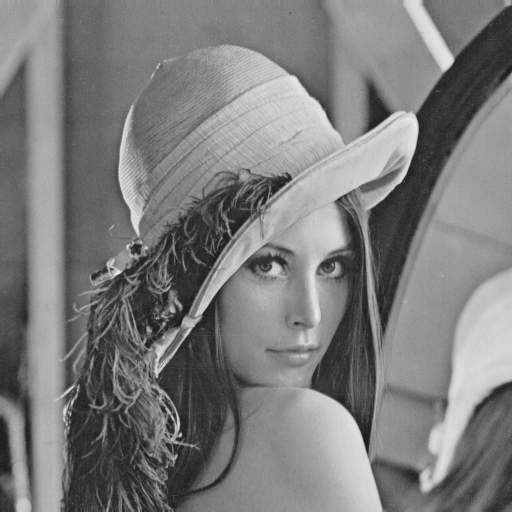
\includegraphics[width=.5\textwidth]{img.png}
\caption{Original Image (Lena)}
\label{fig:img}
\end{figure}

% Equalize -> Filter
\begin{figure}[h]
\centering
\begin{subfigure}{.5\textwidth}
  \centering
  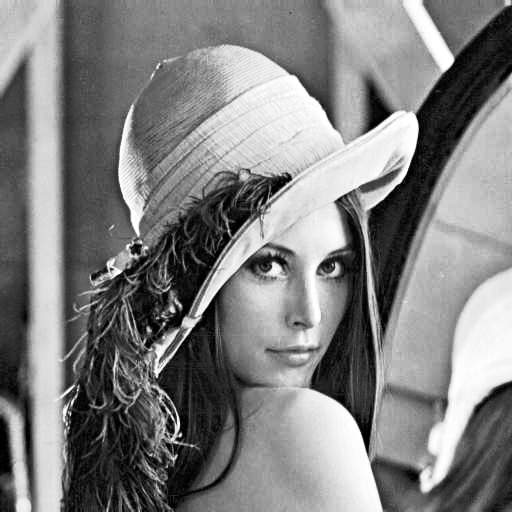
\includegraphics[width=.8\linewidth]{eq.png}
  \caption{Equalized Image}
  \label{fig:eq}
\end{subfigure}%
\begin{subfigure}{.5\textwidth}
  \centering
  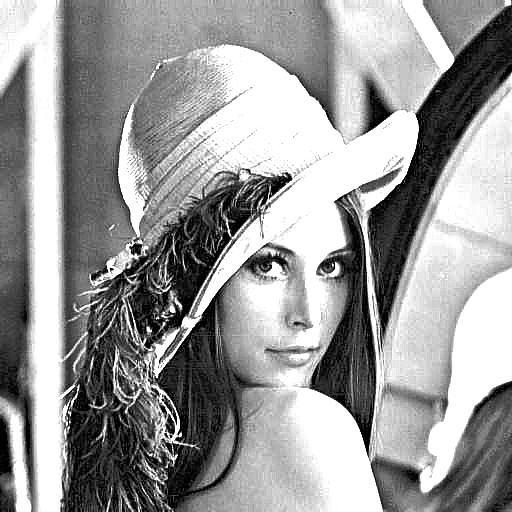
\includegraphics[width=.8\linewidth]{eqFilter.png}
  \caption{Filtered Image after equalization}
  \label{fig:eqFilter}
\end{subfigure}
\caption{Equalize first, then filter}
\label{fig:EqFilter}
\end{figure}

% Filter -> Equalize
\begin{figure}[h]
\centering
\begin{subfigure}{.5\textwidth}
  \centering
  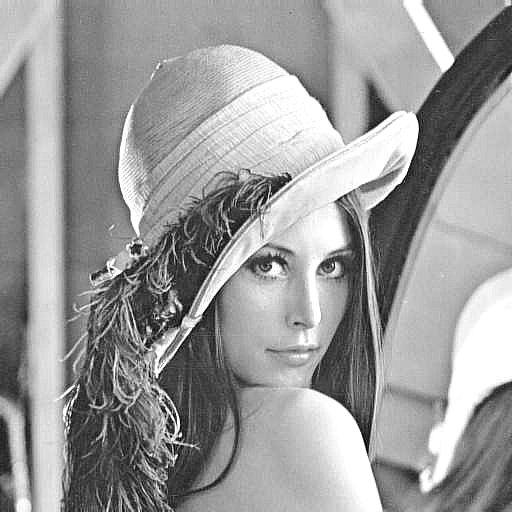
\includegraphics[width=.8\linewidth]{filter.png}
  \caption{Filtered Image}
  \label{fig:filter}
\end{subfigure}%
\begin{subfigure}{.5\textwidth}
  \centering
  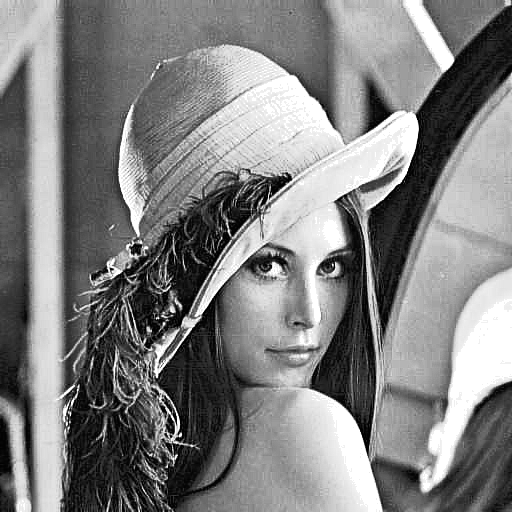
\includegraphics[width=.8\linewidth]{filterEq.png}
  \caption{Equalized Image after filtering}
  \label{fig:filterEq}
\end{subfigure}
\caption{Filter first, then equalize}
\label{fig:FilterEq}
\end{figure}


\end{document}